\subsubsection{Boundry-klasse: PcCom}

\begin{figure}[h]
\centering
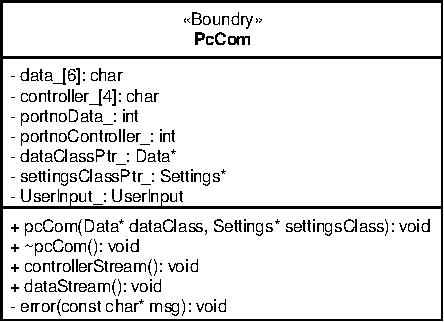
\includegraphics[]{../fig/diagrammer/bil/cd_pccom.pdf}
\caption{Klassebeskrivelse for boundry-klassen PcCom}
\label{fig:cd_pccom}
\end{figure}

\textbf{Attributter}

\begin{table}[h]
\begin{tabularx}{\textwidth}{| Z | Z | L{10cm} |} \hline
Navn & Type & Beskrivelse \\\hline
\texttt{data\_}					& \texttt{char[6]}	&Array af typen char med variable der indeholder hhv. maksimal hastighed, nuværende hastighed, afstand til nærmeste forhindring, nuværende acceleration, AKS status og styretøjs calibrering.\\\hline

\texttt{controller\_}			& \texttt{char[4]}	&Array af typen char med variable der indeholder bruger input for hhv. frem, tilbage, drej og stop.\\\hline

\texttt{portnoData\_}			& \texttt{int}		&Variabel der indeholder portnummeret til den TCP socket der har med overførelse til og fra data\_ array'et.\\\hline

\texttt{portno- Controller\_}	& \texttt{int}		&Variabel der indeholder portnummeret til den TCP socket der har med overførelse til og fra controller\_ array'et.\\\hline

\texttt{dataClassPtr\_}			& \texttt{Data*}	&En pointer til det objekt af typen Data der ønskes læst og skrevet data til.\\\hline

\texttt{settings- ClassPtr\_}	& \texttt{Settings*}&En pointer til det objekt af typen Settings der ønskes skrevet data til.\\\hline

\texttt{UserInput\_}			& \texttt{UserInput}&En struct af typen UserInput der har fire chars, hhv. frem, tilbage, drej og stop.\\\hline
\end{tabularx}
\caption{Attributter for klassen PcCom}
\label{table:attr_pccom}
\end{table}

\clearpage

\textbf{Metoder}

\begin{table}[h]
\begin{tabularx}{\textwidth}{| L{2.5 cm} | Z |} \hline
Prototype 	& \texttt{void PcCom(Data* dataClass, Settings* settingsClass, Log* logClass)} \\\hline
Parametre 	& \texttt{dataClass} 		\newline Det objekt af typen Data der ønskes bearbjedet af PcCom. \newline \newline
			  \texttt{settingsClass} 	\newline Det objekt af typen Settings der ønskes bearbjedet af PcCom. \newline \newline
			  \texttt{logClass}	 		\newline Det objekt af typen Log der ønskes skrevet til af PcCom. \\\hline
Returværdi	& \texttt{void} 			\newline \\\hline
Beskrivelse	& Constructor til klassen PcCom. \newline \\\hline
\end{tabularx}
\caption{Metodebeskrivelse for constructoren af \texttt{PcCom} klassen}
\label{table:met_pccom}
\end{table}

\begin{table}[h]
\begin{tabularx}{\textwidth}{| L{2.5 cm} | Z |} \hline
Prototype 	& \texttt{void $\sim$PcCom()} \\\hline
Parametre 	& \texttt{void}				\newline \\\hline
Returværdi	& \texttt{void} 			\newline \\\hline
Beskrivelse	& Destructor til klassen PcCom. \newline \\\hline
\end{tabularx}
\caption{Metodebeskrivelse for destructoren af \texttt{PcCom} klassen}
\label{table:met_pccom_de}
\end{table}

\begin{table}[h]
\begin{tabularx}{\textwidth}{| L{2.5 cm} | Z |} \hline
Prototype 	& \texttt{void controllerStream()} \\\hline
Parametre 	& \texttt{void}				\newline \\\hline
Returværdi	& \texttt{void} 			\newline \\\hline
Beskrivelse	& Denne funktion har til formål at initialisere og køre en TCP server. Denne server skal streame hhv. frem-, tilbage-, drej- og stop-kommandoer fra PC'en til bilen. Herefter skal den sende den streamede data til Data klassen. \\\hline
\end{tabularx}
\caption{Metodebeskrivelse for \texttt{controllerStream()}}
\label{table:met_controllerstream}
\end{table}

\clearpage

\begin{table}[h]
\begin{tabularx}{\textwidth}{| L{2.5 cm} | Z |} \hline
Prototype 	& \texttt{void dataStream()} \\\hline
Parametre 	& \texttt{void}				\newline \\\hline
Returværdi	& \texttt{void} 			\newline \\\hline
Beskrivelse	& Denne funktion har til formål at initialisere og køre en TCP server. Denne server skal streame hhv. maksimal hastighed, nuværende hastighed, afstand til nærmeste forhindring, nuværende acceleration, AKS status og styretøjs calibrering fra PC'en til bilen. Herefter skal den sende den streamede data til Data og Settings klassen. \\\hline
\end{tabularx}
\caption{Metodebeskrivelse for \texttt{dataStream()}}
\label{table:met_datastream}
\end{table}

\begin{table}[h]
\begin{tabularx}{\textwidth}{| L{2.5 cm} | Z |} \hline
Prototype 	& \texttt{void error(string msg)} \\\hline
Parametre 	& \texttt{msg}				\newline En pågældende fejl-besked i form af en string. \\\hline
Returværdi	& \texttt{void} 			\newline \\\hline
Beskrivelse	& Denne funktion har til formål at skrive en fejl til log, hvis der opstår en fejl. \newline \\\hline
\end{tabularx}
\caption{Metodebeskrivelse for \texttt{error()}}
\label{table:met_error}
\end{table}